% fixture: tikz/tree-grow
% tier: T3
% engine: document
% specials: compare
% covers: TikZ trees' growth (grow and grow' with a direction's name or an angle on the picture, a level and one child: the level whose children are not spread; growth parent anchor; grow siblings on line)
\documentclass{article}
\usepackage{tikz}
\pagestyle{empty}
\begin{document}
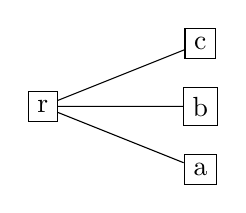
\begin{tikzpicture}[grow=right, level distance=2cm, sibling distance=8mm]
  \node[draw] {r} child { node[draw] {a} } child { node[draw] {b} } child { node[draw] {c} };
\end{tikzpicture}

\begin{tikzpicture}[grow'=up, level 2/.style={grow=30, sibling distance=6mm}, growth parent anchor=north]
  \node {r}
    child { node {a} child { node {d} } child { node {e} } }
    child[grow=left] { node {b} }
    child[grow'=south west, level distance=5mm] { node {c} }
    child[grow siblings on line] { node {f} };
\end{tikzpicture}
\end{document}
